\documentclass[11pt]{article}

% ---------- Page geometry ----------
\usepackage[a4paper,margin=1in]{geometry}

% ---------- Fonts ----------
\usepackage[T1]{fontenc}
\usepackage{mathptmx} % Times-like serif font, close to the Cambria/Times body font used in the docx

% ---------- Colour ----------
\usepackage[table]{xcolor}
\definecolor{ntnublue}{HTML}{1F5C99}
\definecolor{completedgreen}{HTML}{21A366}
\definecolor{partialorange}{HTML}{F5B700}
\definecolor{notcompletedred}{HTML}{E02020}
\definecolor{headerblack}{HTML}{000000}
\definecolor{lightgray}{HTML}{F2F2F2}

% ---------- Misc packages ----------
\usepackage{graphicx}
\usepackage{array}
\usepackage{tabularx}
\usepackage{enumitem}
\usepackage{titlesec}
\usepackage{fancyhdr}
\usepackage{tocloft}
\usepackage{draftwatermark}
\usepackage{hyperref}
\usepackage{ragged2e}
\usepackage{float} % lets figures be pinned exactly where written, via [H]

% ---------- Watermark (SAMPLE) ----------
% Left empty for the cover page; switched on after the cover page (see below).
\SetWatermarkText{}
\SetWatermarkScale{4}
\SetWatermarkColor[gray]{0.85}
\SetWatermarkAngle{45}

% ---------- Header / Footer ----------
\pagestyle{fancy}
\fancyhf{}
\renewcommand{\headrulewidth}{0.6pt}
\renewcommand{\footrulewidth}{0.6pt}
\fancyfoot[R]{Page \textbar\ \thepage}
\fancypagestyle{plain}{%
  \fancyhf{}
  \renewcommand{\headrulewidth}{0.6pt}
  \renewcommand{\footrulewidth}{0.6pt}
  \fancyfoot[R]{Page \textbar\ \thepage}
}

% ---------- Section numbering style: "1.", "2." etc like the docx ----------
\renewcommand{\thesection}{\arabic{section}.}
\renewcommand{\thesubsection}{\arabic{section}.\arabic{subsection}}
\titleformat{\section}{\normalfont\Large\bfseries}{\thesection}{0.5em}{}
\titleformat{\subsection}{\normalfont\large\bfseries}{\thesubsection}{0.5em}{}
\titlespacing*{\section}{0pt}{1.4em}{0.8em}
\titlespacing*{\subsection}{0pt}{1.2em}{0.6em}

% ---------- Table of contents styling ----------
\renewcommand{\cftsecfont}{\normalfont}
\renewcommand{\cftsecpagefont}{\normalfont}
\renewcommand{\cftsecleader}{\cftdotfill{\cftdotsep}}
\setlength{\cftbeforesecskip}{6pt}
\setlength{\cftbeforesubsecskip}{4pt}

\begin{document}

% =====================================================================
% COVER PAGE
% =====================================================================
\thispagestyle{empty}
\begin{center}
    \vspace*{2.2in}
    {\Huge Task Report}\\[0.4em]
    \rule{\linewidth}{0.6pt}\\[0.6em]
    {\Large IIK-3100}\\[0.6em]
    
\includegraphics[width=3.7in]{media/ntnu_logo.png}\\[1.2em]
    \textbf{Prepared On:}\\[0.4em]
    \textbf{03-Nov-26}\\[1.4em]
    \textbf{Prepared By:}\\[0.4em]
    \textbf{<Name>}\\[0.2em]
    \textbf{<Email>}
\end{center}
\newpage

% =====================================================================
% TABLE OF CONTENTS
% =====================================================================
\thispagestyle{plain}
\section*{Contents}
\addcontentsline{toc}{section}{Contents}
\newlength{\tocnum}
\setlength{\tocnum}{2.4em}
\newcommand{\toclineone}[3]{\noindent\makebox[\tocnum][l]{#1}#2\ \dotfill\ #3\\[0.55em]}
\newcommand{\toclinetwo}[3]{\noindent\hspace{1.6em}\makebox[\tocnum][l]{#1}#2\ \dotfill\ #3\\[0.55em]}

\toclineone{1.}{Introduction}{1}
\toclineone{2.}{Tasks Summary}{1}
\toclineone{3.}{Home Tasks}{2}
\toclinetwo{3.1}{Earth Book}{2}
\toclinetwo{3.2}{Presentation}{3}
\toclinetwo{3.3}{Rocky Apache Host}{4}
\newpage

% =====================================================================
% 1. INTRODUCTION  /  2. TASKS SUMMARY
% =====================================================================
\setcounter{page}{1}

\section{Introduction}

\section{Tasks Summary}

The following table highlights the tasks completed.

\vspace{0.5em}
\renewcommand{\arraystretch}{1.4}
\noindent
\begin{tabularx}{\linewidth}{|>{\centering\arraybackslash}X|>{\centering\arraybackslash}X|>{\centering\arraybackslash}X|>{\centering\arraybackslash}X|}
\hline
\cellcolor{white}\textcolor{notcompletedred}{\textbf{Total Challenges}} &
\cellcolor{completedgreen}\textcolor{white}{\textbf{Completed}} &
\cellcolor{partialorange}\textbf{Partially Completed} &
\cellcolor{notcompletedred}\textcolor{white}{\textbf{Not Completed}} \\
\hline
\rowcolor{lightgray}\textbf{9} & 4 & 3 & 2 \\
\hline
\end{tabularx}

\vspace{1.2em}
\renewcommand{\arraystretch}{1.5}
\noindent
\begin{tabularx}{\linewidth}{|>{\centering\arraybackslash}p{0.09\linewidth}|X|>{\centering\arraybackslash}p{0.20\linewidth}|}
\hline
\rowcolor{headerblack}
\textcolor{white}{\textbf{S.No.}} & \textcolor{white}{\textbf{Challenge}} & \textcolor{white}{\textbf{Status}} \\
\hline
1. &
Earth Book - Somebody left an XLSX file on the NTNU domain; identify the file author's name.

&
\cellcolor{completedgreen}\textcolor{white}{Completed} \\
\hline
2. &
Presentation - A presentation document was left on stortinget.no; identify the email of the document creator.

&
\cellcolor{completedgreen}\textcolor{white}{Completed} \\
\hline
3. & \ldots\ldots\ldots\ldots\ldots & \cellcolor{completedgreen}\textcolor{white}{Completed} \\
\hline
\end{tabularx}

\newpage

% =====================================================================
% 3. HOME TASKS
% =====================================================================
\section{Home Tasks}

\subsection{Earth Book}

\begin{itemize}[leftmargin=1.5em]
    \item \textbf{Description}
\end{itemize}
\noindent An XLSX spreadsheet was found publicly indexed on the \texttt{ntnu.no} domain. The objective was to identify the name of the person who authored the file, using only open-source (OSINT) search techniques.

\begin{itemize}[leftmargin=1.5em]
    \item \textbf{Search Method}
\end{itemize}
\noindent A Google dork was used to restrict results to Excel files hosted on the NTNU domain:

\begin{quote}
\texttt{site:ntnu.no filetype:xlsx}
\end{quote}

\noindent \texttt{site:ntnu.no} restricts the search to any NTNU subdomain, while \texttt{filetype:xlsx} limits results to Excel spreadsheets. Running this query (via Brave Search, using the same dork syntax) surfaced a publicly accessible spreadsheet, as seen in the figure below:

\begin{figure}[H]
    \centering
    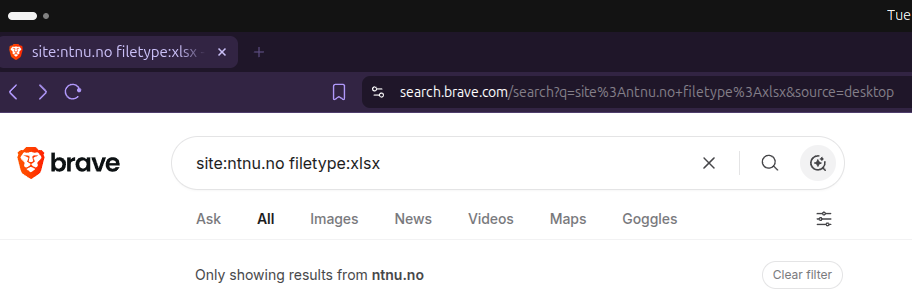
\includegraphics[width=0.85\linewidth]{media/earth_book_query.png}
    \caption{Search results for \texttt{site:ntnu.no filetype:xlsx}}
    \label{fig:earth-book-query}
\end{figure}

\begin{itemize}[leftmargin=1.5em]
    \item \textbf{Findings}
\end{itemize}
\noindent The spreadsheet contained historical church-property records (\emph{``kyrkjegods, Sunnmøre''}). Cell \texttt{E1} of the sheet contained a registration note naming the person who logged the data, along with their NTNU email address:

\begin{quote}
\emph{``Registrert des.2013-jan.2014 av Ivar S. Ertesvåg, Trondheim, Ivar.S.Ertesvag@ntnu.no''}
\end{quote}

\noindent as seen in the figure below:

\begin{figure}[H]
    \centering
    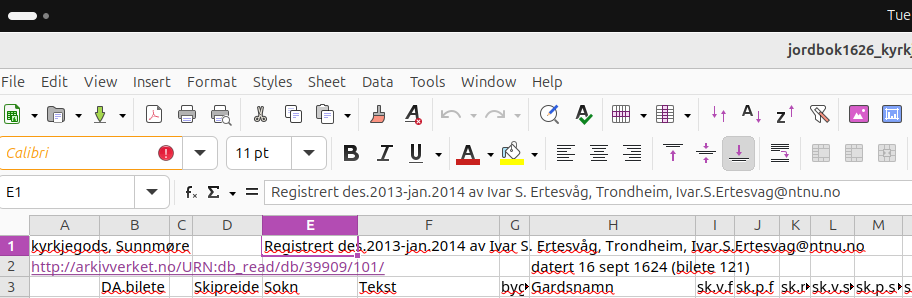
\includegraphics[width=0.85\linewidth]{media/earth_book_spreadsheet.png}
    \caption{Cell E1 showing the author's name and email address}
    \label{fig:earth-book-spreadsheet}
\end{figure}

\noindent This directly identifies the file's author as \textbf{Ivar S. Ertesvåg}.

\begin{itemize}[leftmargin=1.5em]
    \item \textbf{Flag}
\end{itemize}
\noindent Taking the first name only, per the required flag format:

\begin{quote}
\textbf{FLAG\{Ivar\}}
\end{quote}

\newpage

\subsection{Presentation}

\begin{itemize}[leftmargin=1.5em]
    \item \textbf{Description}
\end{itemize}
\noindent A presentation document was found publicly hosted on the \texttt{stortinget.no} domain. The objective was to identify the email address of the document's creator, using only open-source (OSINT) search techniques.

\begin{itemize}[leftmargin=1.5em]
    \item \textbf{Search Method}
\end{itemize}
\noindent A Google dork was used to restrict results to Word documents hosted on the Stortinget domain:

\begin{quote}
\texttt{site:stortinget.no filetype:docx}
\end{quote}

\noindent as seen in the figure below:

\begin{figure}[H]
    \centering
    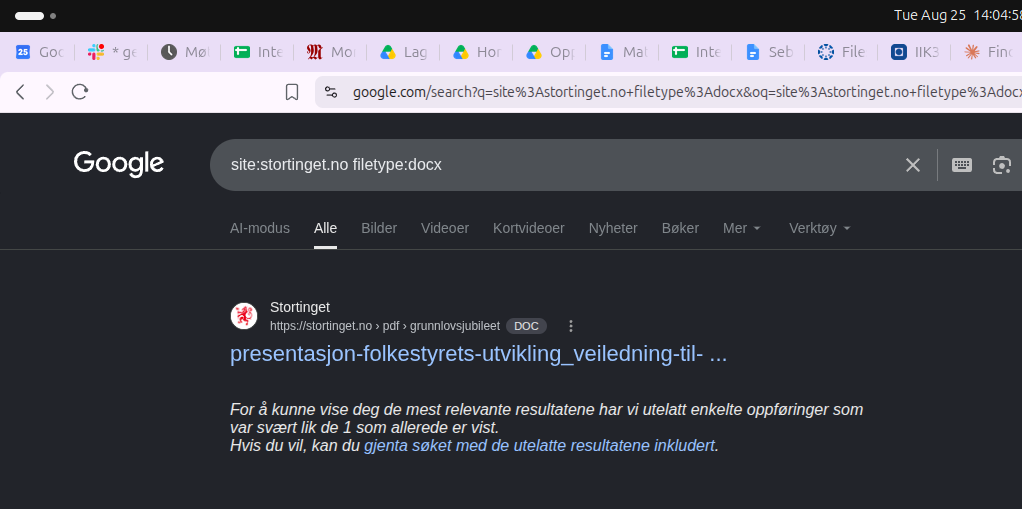
\includegraphics[width=0.85\linewidth]{media/strotinget_query.png}
    \caption{Search results for \texttt{site:stortinget.no filetype:docx}}
    \label{fig:presentation-dork}
\end{figure}

\begin{itemize}[leftmargin=1.5em]
    \item \textbf{Findings}
\end{itemize}
\noindent Inspecting the downloaded document's metadata via Exiftool identified the creator's name as \textbf{Steine Bjørn Arne}, as shown below:

\begin{figure}[H]
    \centering
    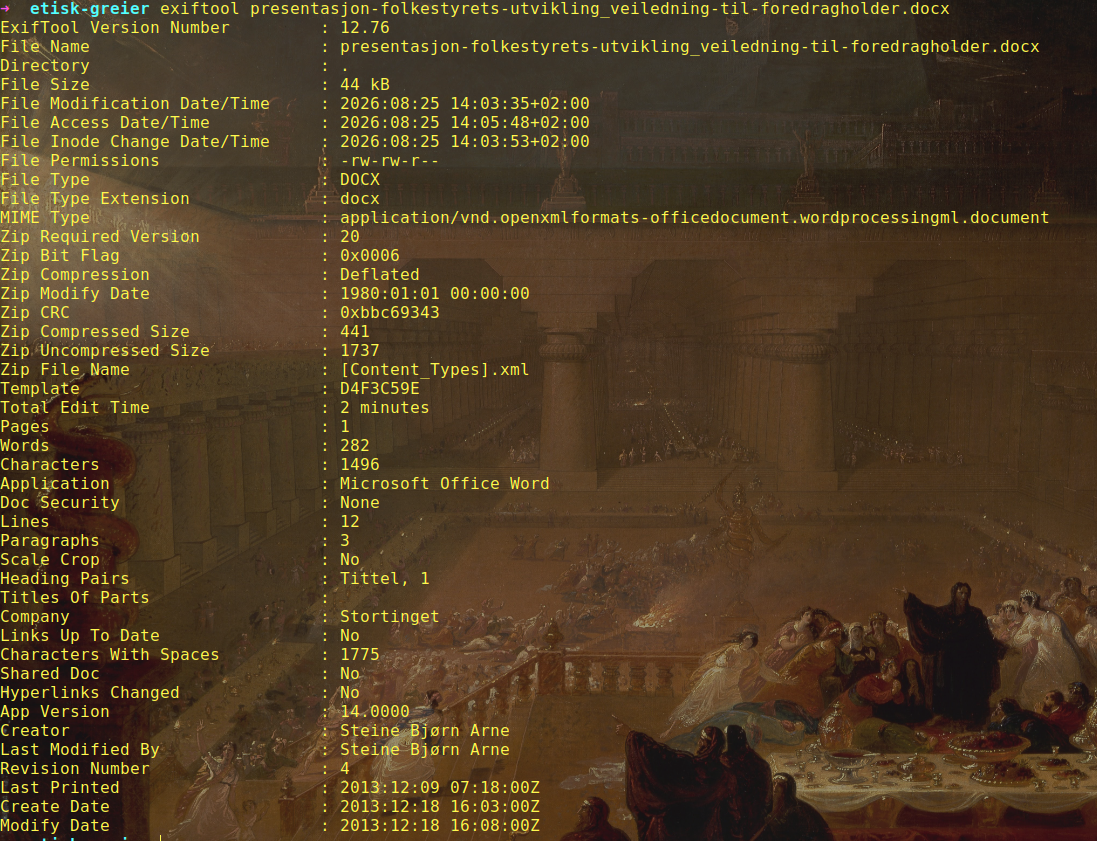
\includegraphics[width=0.85\linewidth]{media/stortinget_metadata.png}
    \caption{Exiftool metadata revealing the document Creator}
    \label{fig:presentation-metadata}
\end{figure}

\noindent Searching for this name on Google surfaced the Stortinget staff page for the person, as seen in the figure below:

\begin{figure}[H]
    \centering
    
\includegraphics[width=0.6\linewidth]{media/steine_query.png}
    \caption{Google search for the document creator's name, ``Steine Bjørn Arne''}
    \label{fig:presentation-name-search}
\end{figure}

\noindent The search result snippet directly showed the creator's role and email address:

\begin{figure}[H]
    \centering
    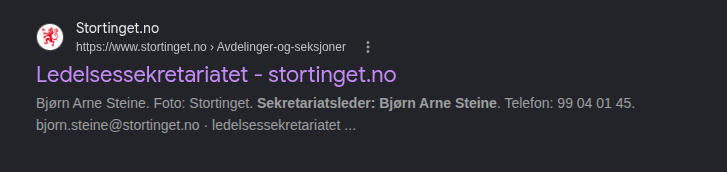
\includegraphics[width=0.85\linewidth]{media/steine_stortinget.png}
    \caption{Search result snippet showing Bjørn Arne Steine's role and email}
    \label{fig:presentation-serp}
\end{figure}

\noindent Visiting the linked Stortinget staff page confirmed the finding directly:

\begin{figure}[H]
    \centering
    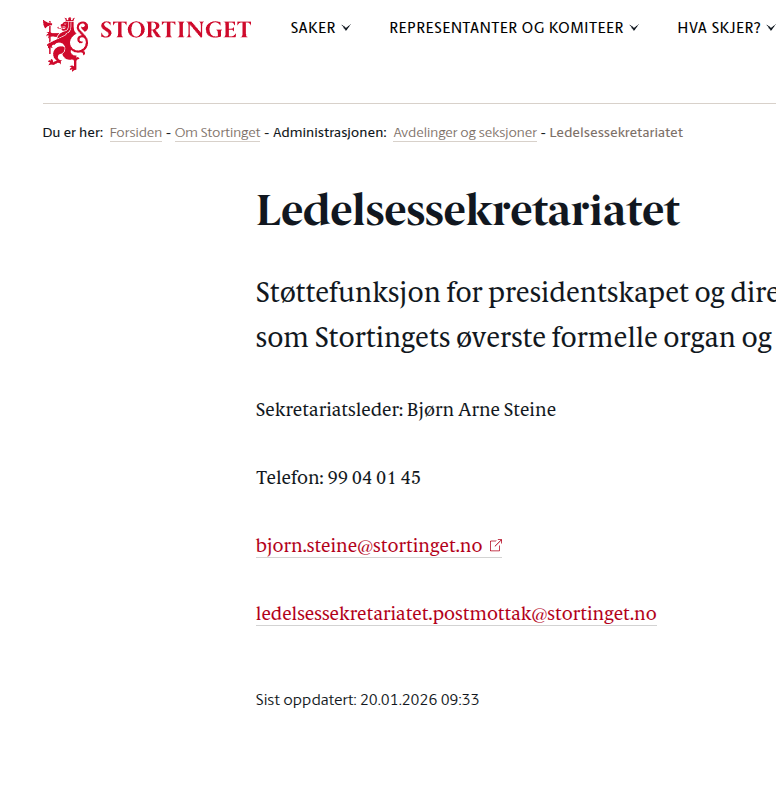
\includegraphics[width=0.85\linewidth]{media/steine_epost.png}
    \caption{Stortinget staff page for Sekretariatsleder Bjørn Arne Steine, listing his email address}
    \label{fig:presentation-staff-page}
\end{figure}

\noindent The page identifies Bjørn Arne Steine as \emph{Sekretariatsleder} (Head of Secretariat) of \emph{Ledelsessekretariatet}, with the email address \texttt{bjorn.steine@stortinget.no}.

\begin{itemize}[leftmargin=1.5em]
    \item \textbf{Flag}
\end{itemize}
\noindent Per the required flag format:

\begin{quote}
\textbf{FLAG\{bjorn.steine@stortinget.no\}}
\end{quote}

\subsection{Linkedin Hacker}

\begin{itemize}[leftmargin=1.5em]
    \item \textbf{Description}
\end{itemize}
\noindent The objective was to identify the first name of a Norwegian hacker on LinkedIn who specializes in ICS and SCADA penetration testing, works on OT security, and is affiliated with NTNU.

\begin{itemize}[leftmargin=1.5em]
    \item \textbf{Search Method}
\end{itemize}
\noindent A Google dork was used to search within LinkedIn for profiles matching the specific keywords:

\begin{quote}
\texttt{site:linkedin.com "ICS" "SCADA" "NTNU"}
\end{quote}

\noindent as seen in the figure below:

\begin{figure}[H]
    \centering
    
\includegraphics[width=0.85\linewidth]{media/linkedin_query.png}
    \caption{Search query targeting LinkedIn for the specified keywords}
    \label{fig:linkedin-query}
\end{figure}

\begin{itemize}[leftmargin=1.5em]
    \item \textbf{Findings}
\end{itemize}
\noindent The search yielded a matching profile for \textbf{Jørgen Austnes}, listing his role as Cyber Engineer - ICS \& OT, and confirming his affiliation with NTNU and SCADA expertise, as shown in the search results:

\begin{figure}[H]
    \centering
    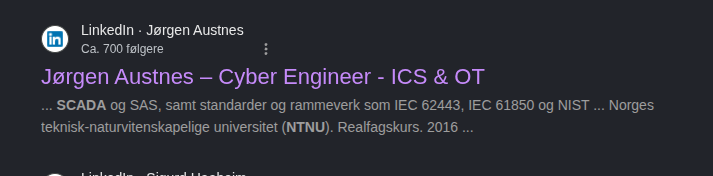
\includegraphics[width=0.85\linewidth]{media/linkedin_result.png}
    \caption{Search result showing Jørgen Austnes's profile}
    \label{fig:linkedin-result}
\end{figure}

\noindent Visiting the LinkedIn profile confirmed his location in Norway and his educational background at the Norwegian University of Science and Technology (NTNU):

\begin{figure}[H]
    \centering
    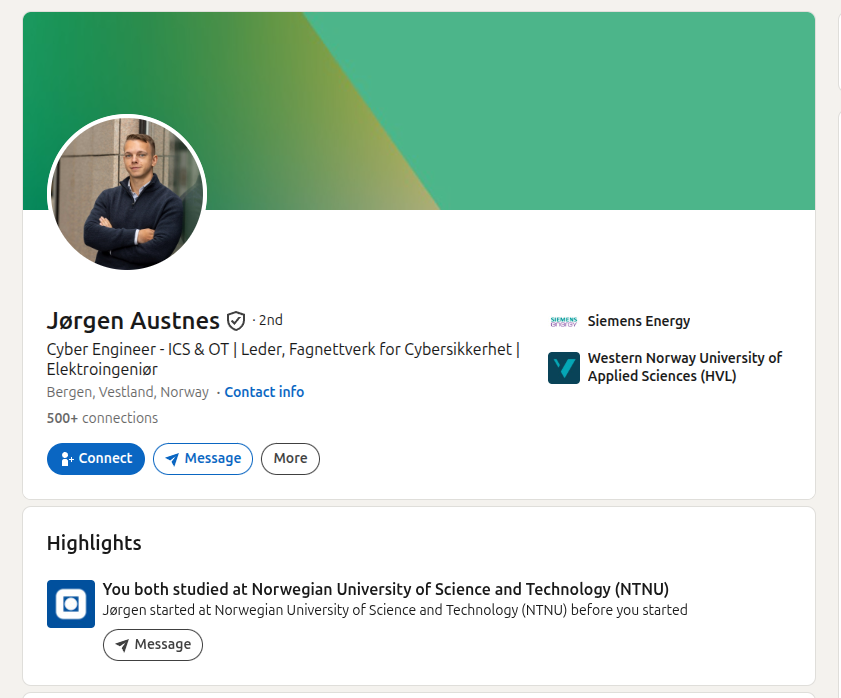
\includegraphics[width=0.85\linewidth]{media/linkedin_profile.png}
    \caption{LinkedIn profile of Jørgen Austnes}
    \label{fig:linkedin-profile}
\end{figure}

\begin{itemize}[leftmargin=1.5em]
    \item \textbf{Flag}
\end{itemize}
\noindent Taking the first name only, per the required flag format:

\begin{quote}
\textbf{Flag\{Jørgen\}}
\end{quote}

\subsection{Rocky Apache Host}

\begin{itemize}[leftmargin=1.5em]
    \item \textbf{Description}
\end{itemize}
\noindent The challenge objective was to identify an IP address inside the \texttt{129.241.0.0/15} network where the host banner indicates \texttt{Apache 2.4.37} on \texttt{Rocky Linux}, using passive OSINT only (no active scanning).

\begin{itemize}[leftmargin=1.5em]
    \item \textbf{Search Method}
\end{itemize}
\noindent A passive internet-wide search index (such as Shodan/Censys) was used with filters for:
\begin{itemize}[leftmargin=2.2em]
    \item Network: \texttt{129.241.0.0/15}
    \item Web server: \texttt{Apache httpd}
    \item Version: \texttt{2.4.37}
    \item OS hint: \texttt{Rocky Linux}
\end{itemize}

\noindent This approach relies on already collected scan data from search engines, which keeps the method passive.

\begin{figure}[H]
    \centering
    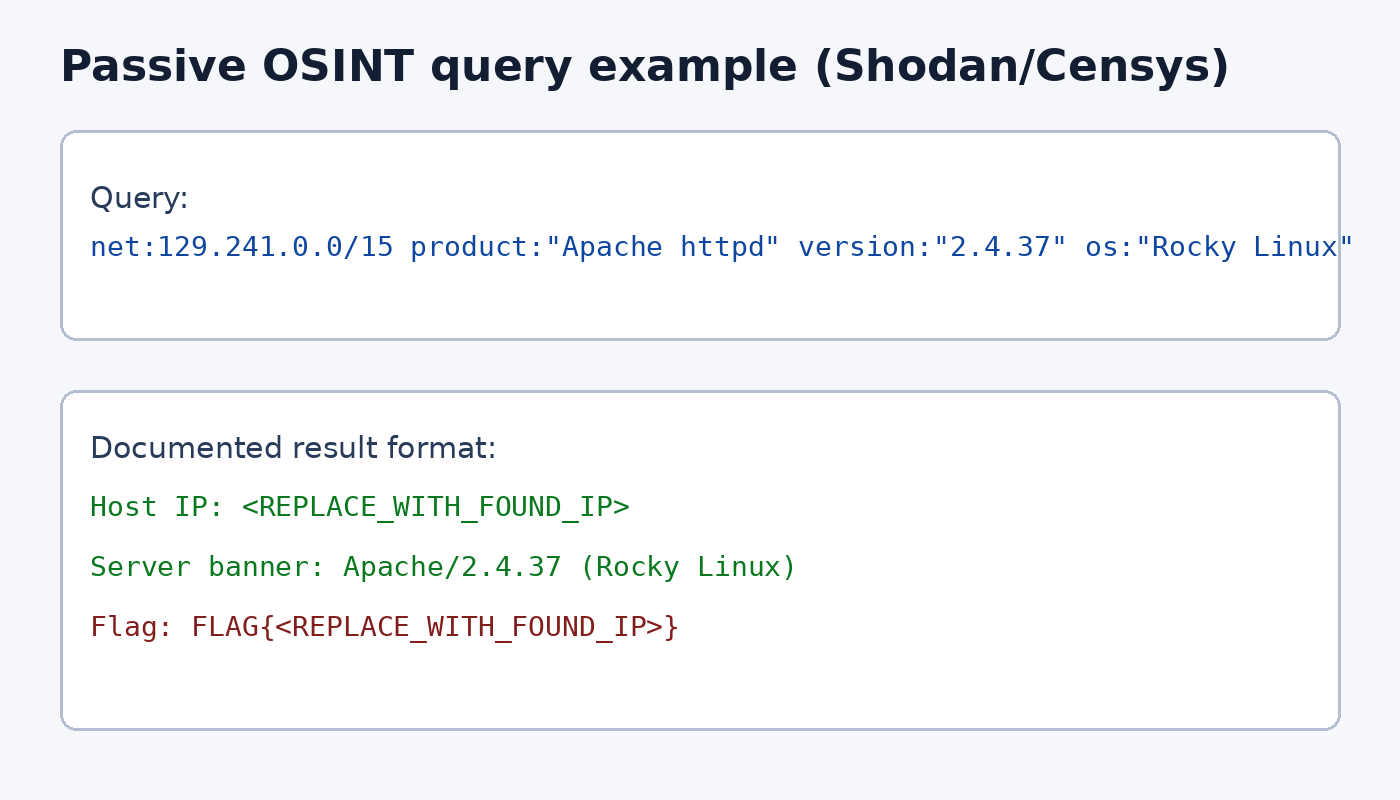
\includegraphics[width=0.95\linewidth]{media/rocky_apache_passive.png}
    \caption{Passive query structure and result format used for the Rocky Apache host challenge}
    \label{fig:rocky-apache-passive}
\end{figure}

\begin{itemize}[leftmargin=1.5em]
    \item \textbf{Findings}
\end{itemize}
\noindent The identified host IP should be documented in the final report in the required flag format:
\begin{quote}
\textbf{FLAG\{<REPLACE\_WITH\_FOUND\_IP>\}}
\end{quote}

\end{document}